\documentclass[twoside]{book}

% Packages required by doxygen
\usepackage{fixltx2e}
\usepackage{calc}
\usepackage{doxygen}
\usepackage{graphicx}
\usepackage[utf8]{inputenc}
\usepackage{makeidx}
\usepackage{multicol}
\usepackage{multirow}
\PassOptionsToPackage{warn}{textcomp}
\usepackage{textcomp}
\usepackage[nointegrals]{wasysym}
\usepackage[table]{xcolor}

% Font selection
\usepackage[T1]{fontenc}
\usepackage{mathptmx}
\usepackage[scaled=.90]{helvet}
\usepackage{courier}
\usepackage{amssymb}
\usepackage{sectsty}
\renewcommand{\familydefault}{\sfdefault}
\allsectionsfont{%
  \fontseries{bc}\selectfont%
  \color{darkgray}%
}
\renewcommand{\DoxyLabelFont}{%
  \fontseries{bc}\selectfont%
  \color{darkgray}%
}
\newcommand{\+}{\discretionary{\mbox{\scriptsize$\hookleftarrow$}}{}{}}

% Page & text layout
\usepackage{geometry}
\geometry{%
  a4paper,%
  top=2.5cm,%
  bottom=2.5cm,%
  left=2.5cm,%
  right=2.5cm%
}
\tolerance=750
\hfuzz=15pt
\hbadness=750
\setlength{\emergencystretch}{15pt}
\setlength{\parindent}{0cm}
\setlength{\parskip}{0.2cm}
\makeatletter
\renewcommand{\paragraph}{%
  \@startsection{paragraph}{4}{0ex}{-1.0ex}{1.0ex}{%
    \normalfont\normalsize\bfseries\SS@parafont%
  }%
}
\renewcommand{\subparagraph}{%
  \@startsection{subparagraph}{5}{0ex}{-1.0ex}{1.0ex}{%
    \normalfont\normalsize\bfseries\SS@subparafont%
  }%
}
\makeatother

% Headers & footers
\usepackage{fancyhdr}
\pagestyle{fancyplain}
\fancyhead[LE]{\fancyplain{}{\bfseries\thepage}}
\fancyhead[CE]{\fancyplain{}{}}
\fancyhead[RE]{\fancyplain{}{\bfseries\leftmark}}
\fancyhead[LO]{\fancyplain{}{\bfseries\rightmark}}
\fancyhead[CO]{\fancyplain{}{}}
\fancyhead[RO]{\fancyplain{}{\bfseries\thepage}}
\fancyfoot[LE]{\fancyplain{}{}}
\fancyfoot[CE]{\fancyplain{}{}}
\fancyfoot[RE]{\fancyplain{}{\bfseries\scriptsize Generated on Mon Oct 3 2016 11\+:13\+:33 for Appli\+Eleve by Doxygen }}
\fancyfoot[LO]{\fancyplain{}{\bfseries\scriptsize Generated on Mon Oct 3 2016 11\+:13\+:33 for Appli\+Eleve by Doxygen }}
\fancyfoot[CO]{\fancyplain{}{}}
\fancyfoot[RO]{\fancyplain{}{}}
\renewcommand{\footrulewidth}{0.4pt}
\renewcommand{\chaptermark}[1]{%
  \markboth{#1}{}%
}
\renewcommand{\sectionmark}[1]{%
  \markright{\thesection\ #1}%
}

% Indices & bibliography
\usepackage{natbib}
\usepackage[titles]{tocloft}
\setcounter{tocdepth}{3}
\setcounter{secnumdepth}{5}
\makeindex

% Hyperlinks (required, but should be loaded last)
\usepackage{ifpdf}
\ifpdf
  \usepackage[pdftex,pagebackref=true]{hyperref}
\else
  \usepackage[ps2pdf,pagebackref=true]{hyperref}
\fi
\hypersetup{%
  colorlinks=true,%
  linkcolor=blue,%
  citecolor=blue,%
  unicode%
}

% Custom commands
\newcommand{\clearemptydoublepage}{%
  \newpage{\pagestyle{empty}\cleardoublepage}%
}


%===== C O N T E N T S =====

\begin{document}

% Titlepage & ToC
\hypersetup{pageanchor=false,
             bookmarks=true,
             bookmarksnumbered=true,
             pdfencoding=unicode
            }
\pagenumbering{roman}
\begin{titlepage}
\vspace*{7cm}
\begin{center}%
{\Large Appli\+Eleve }\\
\vspace*{1cm}
{\large Generated by Doxygen 1.8.8}\\
\vspace*{0.5cm}
{\small Mon Oct 3 2016 11:13:33}\\
\end{center}
\end{titlepage}
\clearemptydoublepage
\tableofcontents
\clearemptydoublepage
\pagenumbering{arabic}
\hypersetup{pageanchor=true}

%--- Begin generated contents ---
\chapter{Class Index}
\section{Class List}
Here are the classes, structs, unions and interfaces with brief descriptions\+:\begin{DoxyCompactList}
\item\contentsline{section}{\hyperlink{class_eleves}{Eleves} }{\pageref{class_eleves}}{}
\item\contentsline{section}{\hyperlink{class_evaluations}{Evaluations} }{\pageref{class_evaluations}}{}
\item\contentsline{section}{\hyperlink{class_matiere}{Matiere} }{\pageref{class_matiere}}{}
\item\contentsline{section}{\hyperlink{class_notes}{Notes} }{\pageref{class_notes}}{}
\item\contentsline{section}{\hyperlink{class_section}{Section} }{\pageref{class_section}}{}
\end{DoxyCompactList}

\chapter{File Index}
\section{File List}
Here is a list of all files with brief descriptions\+:\begin{DoxyCompactList}
\item\contentsline{section}{\hyperlink{eleves_8cpp}{eleves.\+cpp} }{\pageref{eleves_8cpp}}{}
\item\contentsline{section}{\hyperlink{eleves_8h}{eleves.\+h} }{\pageref{eleves_8h}}{}
\item\contentsline{section}{\hyperlink{_evaluations_8cpp}{Evaluations.\+cpp} }{\pageref{_evaluations_8cpp}}{}
\item\contentsline{section}{\hyperlink{_evaluations_8h}{Evaluations.\+h} }{\pageref{_evaluations_8h}}{}
\item\contentsline{section}{\hyperlink{main_8cpp}{main.\+cpp} }{\pageref{main_8cpp}}{}
\item\contentsline{section}{\hyperlink{_matiere_8cpp}{Matiere.\+cpp} }{\pageref{_matiere_8cpp}}{}
\item\contentsline{section}{\hyperlink{_matiere_8h}{Matiere.\+h} }{\pageref{_matiere_8h}}{}
\item\contentsline{section}{\hyperlink{_notes_8cpp}{Notes.\+cpp} }{\pageref{_notes_8cpp}}{}
\item\contentsline{section}{\hyperlink{_notes_8h}{Notes.\+h} }{\pageref{_notes_8h}}{}
\item\contentsline{section}{\hyperlink{_section_8cpp}{Section.\+cpp} }{\pageref{_section_8cpp}}{}
\item\contentsline{section}{\hyperlink{_section_8h}{Section.\+h} }{\pageref{_section_8h}}{}
\end{DoxyCompactList}

\chapter{Class Documentation}
\hypertarget{class_eleves}{\section{Eleves Class Reference}
\label{class_eleves}\index{Eleves@{Eleves}}
}


{\ttfamily \#include $<$eleves.\+h$>$}



Collaboration diagram for Eleves\+:\nopagebreak
\begin{figure}[H]
\begin{center}
\leavevmode
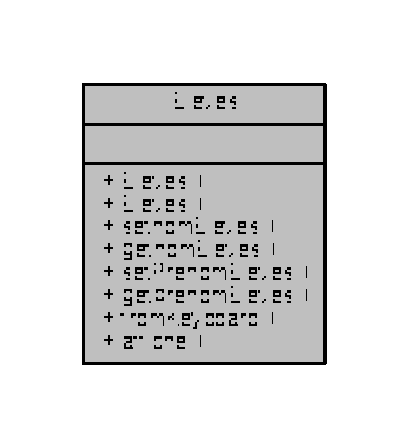
\includegraphics[width=196pt]{class_eleves__coll__graph}
\end{center}
\end{figure}
\subsection*{Public Member Functions}
\begin{DoxyCompactItemize}
\item 
\hyperlink{class_eleves_a1dedbccd0a95ba6af0db2f1d49055f50}{Eleves} ()
\item 
\hyperlink{class_eleves_ad98d50a78df14a3bf88d42e3b0f4d4af}{Eleves} (string lenom\+Eleves, string leprenom\+Eleves)
\item 
void \hyperlink{class_eleves_a9c240aaf34139c8b5a042482827fbe2d}{setnom\+Eleves} (string lenom\+Eleves)
\begin{DoxyCompactList}\small\item\em Initialise la valeur de nom\+Eleves. \end{DoxyCompactList}\item 
string \hyperlink{class_eleves_a00bf5edb75314e55efe8c697fbd5fbcd}{getnom\+Eleves} ()
\item 
void \hyperlink{class_eleves_a97f03e467cadd86e4e46445569559694}{set\+Prenom\+Eleves} (string leprenom\+Eleves)
\begin{DoxyCompactList}\small\item\em Initialise la valeur de prenom\+Eleves. \end{DoxyCompactList}\item 
string \hyperlink{class_eleves_a908388f75621ff9832e9830b31d09c45}{getprenom\+Eleves} ()
\item 
void \hyperlink{class_eleves_ae47e80b391d72d89e4925c15aa74e077}{from\+Keyboard} ()
\begin{DoxyCompactList}\small\item\em saisie d'un élève Permet à l'utilisateur de saisir les valeurs de l'élève \end{DoxyCompactList}\item 
void \hyperlink{class_eleves_a94f519fbb4d38bce24b51baf6f496eb6}{affiche} ()
\begin{DoxyCompactList}\small\item\em affiche info élève Affiche à l'utilisateur le nom et le prénom de l'élève \end{DoxyCompactList}\end{DoxyCompactItemize}


\subsection{Constructor \& Destructor Documentation}
\hypertarget{class_eleves_a1dedbccd0a95ba6af0db2f1d49055f50}{\index{Eleves@{Eleves}!Eleves@{Eleves}}
\index{Eleves@{Eleves}!Eleves@{Eleves}}
\subsubsection[{Eleves}]{\setlength{\rightskip}{0pt plus 5cm}Eleves\+::\+Eleves (
\begin{DoxyParamCaption}
{}
\end{DoxyParamCaption}
)}}\label{class_eleves_a1dedbccd0a95ba6af0db2f1d49055f50}
Empty Constructor \hypertarget{class_eleves_ad98d50a78df14a3bf88d42e3b0f4d4af}{\index{Eleves@{Eleves}!Eleves@{Eleves}}
\index{Eleves@{Eleves}!Eleves@{Eleves}}
\subsubsection[{Eleves}]{\setlength{\rightskip}{0pt plus 5cm}Eleves\+::\+Eleves (
\begin{DoxyParamCaption}
\item[{string}]{lenom\+Eleves, }
\item[{string}]{leprenom\+Eleves}
\end{DoxyParamCaption}
)}}\label{class_eleves_ad98d50a78df14a3bf88d42e3b0f4d4af}


\subsection{Member Function Documentation}
\hypertarget{class_eleves_a94f519fbb4d38bce24b51baf6f496eb6}{\index{Eleves@{Eleves}!affiche@{affiche}}
\index{affiche@{affiche}!Eleves@{Eleves}}
\subsubsection[{affiche}]{\setlength{\rightskip}{0pt plus 5cm}void Eleves\+::affiche (
\begin{DoxyParamCaption}
{}
\end{DoxyParamCaption}
)}}\label{class_eleves_a94f519fbb4d38bce24b51baf6f496eb6}


affiche info élève Affiche à l'utilisateur le nom et le prénom de l'élève 

\hypertarget{class_eleves_ae47e80b391d72d89e4925c15aa74e077}{\index{Eleves@{Eleves}!from\+Keyboard@{from\+Keyboard}}
\index{from\+Keyboard@{from\+Keyboard}!Eleves@{Eleves}}
\subsubsection[{from\+Keyboard}]{\setlength{\rightskip}{0pt plus 5cm}void Eleves\+::from\+Keyboard (
\begin{DoxyParamCaption}
{}
\end{DoxyParamCaption}
)}}\label{class_eleves_ae47e80b391d72d89e4925c15aa74e077}


saisie d'un élève Permet à l'utilisateur de saisir les valeurs de l'élève 



Here is the caller graph for this function\+:\nopagebreak
\begin{figure}[H]
\begin{center}
\leavevmode
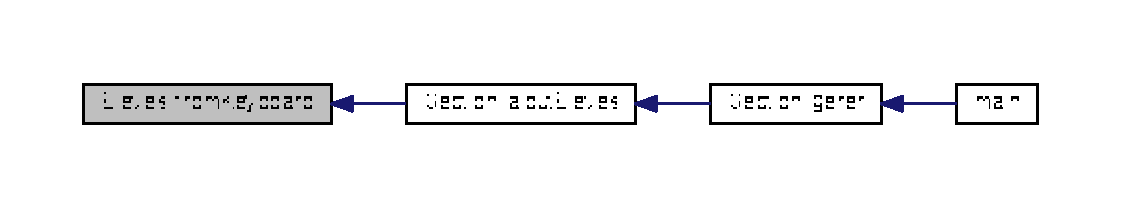
\includegraphics[width=350pt]{class_eleves_ae47e80b391d72d89e4925c15aa74e077_icgraph}
\end{center}
\end{figure}


\hypertarget{class_eleves_a00bf5edb75314e55efe8c697fbd5fbcd}{\index{Eleves@{Eleves}!getnom\+Eleves@{getnom\+Eleves}}
\index{getnom\+Eleves@{getnom\+Eleves}!Eleves@{Eleves}}
\subsubsection[{getnom\+Eleves}]{\setlength{\rightskip}{0pt plus 5cm}string Eleves\+::getnom\+Eleves (
\begin{DoxyParamCaption}
{}
\end{DoxyParamCaption}
)}}\label{class_eleves_a00bf5edb75314e55efe8c697fbd5fbcd}
\begin{DoxyReturn}{Returns}
la valeur de nom\+Eleves
\end{DoxyReturn}
Retourne la valeur de la propriété nom\+Eleves

Get the value of nom\+Eleves \begin{DoxyReturn}{Returns}
the value of nom\+Eleves 
\end{DoxyReturn}
\hypertarget{class_eleves_a908388f75621ff9832e9830b31d09c45}{\index{Eleves@{Eleves}!getprenom\+Eleves@{getprenom\+Eleves}}
\index{getprenom\+Eleves@{getprenom\+Eleves}!Eleves@{Eleves}}
\subsubsection[{getprenom\+Eleves}]{\setlength{\rightskip}{0pt plus 5cm}string Eleves\+::getprenom\+Eleves (
\begin{DoxyParamCaption}
{}
\end{DoxyParamCaption}
)}}\label{class_eleves_a908388f75621ff9832e9830b31d09c45}
\begin{DoxyReturn}{Returns}
la valeur de prenom\+Eleves
\end{DoxyReturn}
Retourne la valeur de la propriété prenom\+Eleves

Get the value of prenom\+Eleves \begin{DoxyReturn}{Returns}
the value of prenom\+Eleves 
\end{DoxyReturn}
\hypertarget{class_eleves_a9c240aaf34139c8b5a042482827fbe2d}{\index{Eleves@{Eleves}!setnom\+Eleves@{setnom\+Eleves}}
\index{setnom\+Eleves@{setnom\+Eleves}!Eleves@{Eleves}}
\subsubsection[{setnom\+Eleves}]{\setlength{\rightskip}{0pt plus 5cm}void Eleves\+::setnom\+Eleves (
\begin{DoxyParamCaption}
\item[{string}]{lenom\+Eleves}
\end{DoxyParamCaption}
)}}\label{class_eleves_a9c240aaf34139c8b5a042482827fbe2d}


Initialise la valeur de nom\+Eleves. 


\begin{DoxyParams}{Parameters}
{\em lenom\+Eleves} & reçoit nom\+Eleves\\
\hline
\end{DoxyParams}
Set the value of nom\+Eleves 
\begin{DoxyParams}{Parameters}
{\em lenom\+Eleves} & the new value of nom\+Eleves \\
\hline
\end{DoxyParams}
\hypertarget{class_eleves_a97f03e467cadd86e4e46445569559694}{\index{Eleves@{Eleves}!set\+Prenom\+Eleves@{set\+Prenom\+Eleves}}
\index{set\+Prenom\+Eleves@{set\+Prenom\+Eleves}!Eleves@{Eleves}}
\subsubsection[{set\+Prenom\+Eleves}]{\setlength{\rightskip}{0pt plus 5cm}void Eleves\+::set\+Prenom\+Eleves (
\begin{DoxyParamCaption}
\item[{string}]{leprenom\+Eleves}
\end{DoxyParamCaption}
)}}\label{class_eleves_a97f03e467cadd86e4e46445569559694}


Initialise la valeur de prenom\+Eleves. 


\begin{DoxyParams}{Parameters}
{\em leprenom\+Eleves} & reçoit prenom\+Eleves\\
\hline
\end{DoxyParams}
Set the value of prenom\+Eleves 
\begin{DoxyParams}{Parameters}
{\em leprenom\+Eleves} & the new value of prenom\+Eleves \\
\hline
\end{DoxyParams}


The documentation for this class was generated from the following files\+:\begin{DoxyCompactItemize}
\item 
\hyperlink{eleves_8h}{eleves.\+h}\item 
\hyperlink{eleves_8cpp}{eleves.\+cpp}\end{DoxyCompactItemize}

\hypertarget{class_evaluations}{\section{Evaluations Class Reference}
\label{class_evaluations}\index{Evaluations@{Evaluations}}
}


{\ttfamily \#include $<$Evaluations.\+h$>$}



Collaboration diagram for Evaluations\+:\nopagebreak
\begin{figure}[H]
\begin{center}
\leavevmode
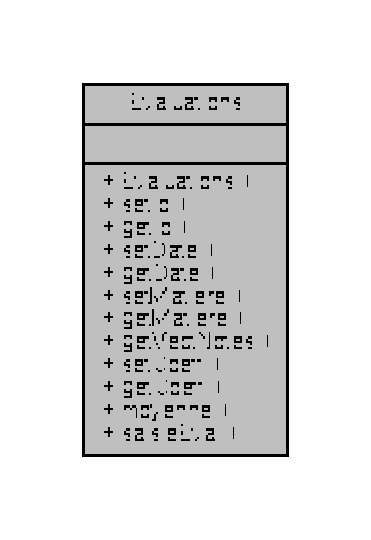
\includegraphics[width=178pt]{class_evaluations__coll__graph}
\end{center}
\end{figure}
\subsection*{Public Member Functions}
\begin{DoxyCompactItemize}
\item 
\hyperlink{class_evaluations_a39ff3292c509ccd40f3ae6ff1cabdcdc}{Evaluations} ()
\item 
void \hyperlink{class_evaluations_a4c7fa1184ee01cfd86a23f3a3050f0af}{set\+Id} (int id\+Eval)
\begin{DoxyCompactList}\small\item\em Initialise la valeur de id. \end{DoxyCompactList}\item 
int \hyperlink{class_evaluations_af9e13687ffeaa9a3197b38aa3777332b}{get\+Id} ()
\item 
void \hyperlink{class_evaluations_a91fa36ac406432cc0654e3931816ae9a}{set\+Date} (string la\+Date)
\begin{DoxyCompactList}\small\item\em Initialise la valeur de date. \end{DoxyCompactList}\item 
string \hyperlink{class_evaluations_ad1d9aafa1b0fe8999a6315194db6ead5}{get\+Date} ()
\item 
void \hyperlink{class_evaluations_af2fdf8aecb0c90fa657fc16cfc284d5c}{set\+Matiere} (\hyperlink{class_matiere}{Matiere} $\ast$la\+Matiere)
\begin{DoxyCompactList}\small\item\em Initialise la valeur de matiere. \end{DoxyCompactList}\item 
\hyperlink{class_matiere}{Matiere} $\ast$ \hyperlink{class_evaluations_a71be15e875c9430528f0f5af9130be21}{get\+Matiere} ()
\item 
vector$<$ \hyperlink{class_notes}{Notes} $>$ \hyperlink{class_evaluations_a3b6e0ec91214a1684914e17ac07fd976}{get\+Vect\+Notes} ()
\begin{DoxyCompactList}\small\item\em vecteur de \hyperlink{class_notes}{Notes} \end{DoxyCompactList}\item 
void \hyperlink{class_evaluations_a06a452d21a1bb0e89bda2ba9b0de9e71}{set\+Coeff} (int le\+Coeff)
\begin{DoxyCompactList}\small\item\em Initialise la valeur de coeff. \end{DoxyCompactList}\item 
int \hyperlink{class_evaluations_a9d6448d35db87f1739735c326e7c1a12}{get\+Coeff} ()
\item 
double \hyperlink{class_evaluations_ab4c0434074b5c060092e7aea29248aed}{moyenne} ()
\begin{DoxyCompactList}\small\item\em Calcul moyenne. \end{DoxyCompactList}\item 
void \hyperlink{class_evaluations_a2e16ac9873e38a0b1d00a9691a9dd95b}{saisie\+Eval} ()
\begin{DoxyCompactList}\small\item\em saisie d'une éval Permet de saisir une évaluation \end{DoxyCompactList}\end{DoxyCompactItemize}


\subsection{Detailed Description}
class \hyperlink{class_evaluations}{Evaluations} 

\subsection{Constructor \& Destructor Documentation}
\hypertarget{class_evaluations_a39ff3292c509ccd40f3ae6ff1cabdcdc}{\index{Evaluations@{Evaluations}!Evaluations@{Evaluations}}
\index{Evaluations@{Evaluations}!Evaluations@{Evaluations}}
\subsubsection[{Evaluations}]{\setlength{\rightskip}{0pt plus 5cm}Evaluations\+::\+Evaluations (
\begin{DoxyParamCaption}
{}
\end{DoxyParamCaption}
)}}\label{class_evaluations_a39ff3292c509ccd40f3ae6ff1cabdcdc}
Empty Constructor 

\subsection{Member Function Documentation}
\hypertarget{class_evaluations_a9d6448d35db87f1739735c326e7c1a12}{\index{Evaluations@{Evaluations}!get\+Coeff@{get\+Coeff}}
\index{get\+Coeff@{get\+Coeff}!Evaluations@{Evaluations}}
\subsubsection[{get\+Coeff}]{\setlength{\rightskip}{0pt plus 5cm}int Evaluations\+::get\+Coeff (
\begin{DoxyParamCaption}
{}
\end{DoxyParamCaption}
)}}\label{class_evaluations_a9d6448d35db87f1739735c326e7c1a12}
\begin{DoxyReturn}{Returns}
le\+Coeff de coeff retourne la valeur de la propriété coeff
\end{DoxyReturn}
Get the value of coeff \begin{DoxyReturn}{Returns}
the value of coeff 
\end{DoxyReturn}
\hypertarget{class_evaluations_ad1d9aafa1b0fe8999a6315194db6ead5}{\index{Evaluations@{Evaluations}!get\+Date@{get\+Date}}
\index{get\+Date@{get\+Date}!Evaluations@{Evaluations}}
\subsubsection[{get\+Date}]{\setlength{\rightskip}{0pt plus 5cm}string Evaluations\+::get\+Date (
\begin{DoxyParamCaption}
{}
\end{DoxyParamCaption}
)}}\label{class_evaluations_ad1d9aafa1b0fe8999a6315194db6ead5}
\begin{DoxyReturn}{Returns}
la\+Date de date retourne la valeur de la propriété date 
\end{DoxyReturn}
\hypertarget{class_evaluations_af9e13687ffeaa9a3197b38aa3777332b}{\index{Evaluations@{Evaluations}!get\+Id@{get\+Id}}
\index{get\+Id@{get\+Id}!Evaluations@{Evaluations}}
\subsubsection[{get\+Id}]{\setlength{\rightskip}{0pt plus 5cm}int Evaluations\+::get\+Id (
\begin{DoxyParamCaption}
{}
\end{DoxyParamCaption}
)}}\label{class_evaluations_af9e13687ffeaa9a3197b38aa3777332b}
\begin{DoxyReturn}{Returns}
id\+Eval de id retourne la valeur de la propriété id
\end{DoxyReturn}
Get the value of id \begin{DoxyReturn}{Returns}
the value of id 
\end{DoxyReturn}
\hypertarget{class_evaluations_a71be15e875c9430528f0f5af9130be21}{\index{Evaluations@{Evaluations}!get\+Matiere@{get\+Matiere}}
\index{get\+Matiere@{get\+Matiere}!Evaluations@{Evaluations}}
\subsubsection[{get\+Matiere}]{\setlength{\rightskip}{0pt plus 5cm}{\bf Matiere} $\ast$ Evaluations\+::get\+Matiere (
\begin{DoxyParamCaption}
{}
\end{DoxyParamCaption}
)}}\label{class_evaluations_a71be15e875c9430528f0f5af9130be21}
\begin{DoxyReturn}{Returns}
la\+Matiere de \hyperlink{class_matiere}{Matiere} retourne la valeur de la propriété \hyperlink{class_matiere}{Matiere}
\end{DoxyReturn}
Get the value of matiere \begin{DoxyReturn}{Returns}
the value of matiere 
\end{DoxyReturn}
\hypertarget{class_evaluations_a3b6e0ec91214a1684914e17ac07fd976}{\index{Evaluations@{Evaluations}!get\+Vect\+Notes@{get\+Vect\+Notes}}
\index{get\+Vect\+Notes@{get\+Vect\+Notes}!Evaluations@{Evaluations}}
\subsubsection[{get\+Vect\+Notes}]{\setlength{\rightskip}{0pt plus 5cm}vector$<$ {\bf Notes} $>$ Evaluations\+::get\+Vect\+Notes (
\begin{DoxyParamCaption}
{}
\end{DoxyParamCaption}
)}}\label{class_evaluations_a3b6e0ec91214a1684914e17ac07fd976}


vecteur de \hyperlink{class_notes}{Notes} 

\begin{DoxyReturn}{Returns}
vect\+Notes retourne le vecteur de \hyperlink{class_notes}{Notes}
\end{DoxyReturn}
Get the value of vec\+Note \begin{DoxyReturn}{Returns}
the value of vec\+Note 
\end{DoxyReturn}
\hypertarget{class_evaluations_ab4c0434074b5c060092e7aea29248aed}{\index{Evaluations@{Evaluations}!moyenne@{moyenne}}
\index{moyenne@{moyenne}!Evaluations@{Evaluations}}
\subsubsection[{moyenne}]{\setlength{\rightskip}{0pt plus 5cm}double Evaluations\+::moyenne (
\begin{DoxyParamCaption}
{}
\end{DoxyParamCaption}
)}}\label{class_evaluations_ab4c0434074b5c060092e7aea29248aed}


Calcul moyenne. 

\begin{DoxyReturn}{Returns}
resultat de moyenne retourne le résultat de la moyenne 
\end{DoxyReturn}
\hypertarget{class_evaluations_a2e16ac9873e38a0b1d00a9691a9dd95b}{\index{Evaluations@{Evaluations}!saisie\+Eval@{saisie\+Eval}}
\index{saisie\+Eval@{saisie\+Eval}!Evaluations@{Evaluations}}
\subsubsection[{saisie\+Eval}]{\setlength{\rightskip}{0pt plus 5cm}void Evaluations\+::saisie\+Eval (
\begin{DoxyParamCaption}
{}
\end{DoxyParamCaption}
)}}\label{class_evaluations_a2e16ac9873e38a0b1d00a9691a9dd95b}


saisie d'une éval Permet de saisir une évaluation 

\hypertarget{class_evaluations_a06a452d21a1bb0e89bda2ba9b0de9e71}{\index{Evaluations@{Evaluations}!set\+Coeff@{set\+Coeff}}
\index{set\+Coeff@{set\+Coeff}!Evaluations@{Evaluations}}
\subsubsection[{set\+Coeff}]{\setlength{\rightskip}{0pt plus 5cm}void Evaluations\+::set\+Coeff (
\begin{DoxyParamCaption}
\item[{int}]{le\+Coeff}
\end{DoxyParamCaption}
)}}\label{class_evaluations_a06a452d21a1bb0e89bda2ba9b0de9e71}


Initialise la valeur de coeff. 


\begin{DoxyParams}{Parameters}
{\em le\+Coeff} & reçoit coeff\\
\hline
\end{DoxyParams}
Set the value of coeff 
\begin{DoxyParams}{Parameters}
{\em new\+\_\+var} & the new value of coeff \\
\hline
\end{DoxyParams}
\hypertarget{class_evaluations_a91fa36ac406432cc0654e3931816ae9a}{\index{Evaluations@{Evaluations}!set\+Date@{set\+Date}}
\index{set\+Date@{set\+Date}!Evaluations@{Evaluations}}
\subsubsection[{set\+Date}]{\setlength{\rightskip}{0pt plus 5cm}void Evaluations\+::set\+Date (
\begin{DoxyParamCaption}
\item[{string}]{la\+Date}
\end{DoxyParamCaption}
)}}\label{class_evaluations_a91fa36ac406432cc0654e3931816ae9a}


Initialise la valeur de date. 


\begin{DoxyParams}{Parameters}
{\em la\+Date} & reçoit date \\
\hline
\end{DoxyParams}
\hypertarget{class_evaluations_a4c7fa1184ee01cfd86a23f3a3050f0af}{\index{Evaluations@{Evaluations}!set\+Id@{set\+Id}}
\index{set\+Id@{set\+Id}!Evaluations@{Evaluations}}
\subsubsection[{set\+Id}]{\setlength{\rightskip}{0pt plus 5cm}void Evaluations\+::set\+Id (
\begin{DoxyParamCaption}
\item[{int}]{id\+Eval}
\end{DoxyParamCaption}
)}}\label{class_evaluations_a4c7fa1184ee01cfd86a23f3a3050f0af}


Initialise la valeur de id. 


\begin{DoxyParams}{Parameters}
{\em id\+Eval} & reçoit id\\
\hline
\end{DoxyParams}
Set the value of id 
\begin{DoxyParams}{Parameters}
{\em new\+\_\+var} & the new value of id \\
\hline
\end{DoxyParams}
\hypertarget{class_evaluations_af2fdf8aecb0c90fa657fc16cfc284d5c}{\index{Evaluations@{Evaluations}!set\+Matiere@{set\+Matiere}}
\index{set\+Matiere@{set\+Matiere}!Evaluations@{Evaluations}}
\subsubsection[{set\+Matiere}]{\setlength{\rightskip}{0pt plus 5cm}void Evaluations\+::set\+Matiere (
\begin{DoxyParamCaption}
\item[{{\bf Matiere} $\ast$}]{la\+Matiere}
\end{DoxyParamCaption}
)}}\label{class_evaluations_af2fdf8aecb0c90fa657fc16cfc284d5c}


Initialise la valeur de matiere. 


\begin{DoxyParams}{Parameters}
{\em la\+Matiere} & reçoit matiere\\
\hline
\end{DoxyParams}
Set the value of matiere 
\begin{DoxyParams}{Parameters}
{\em new\+\_\+var} & the new value of matiere \\
\hline
\end{DoxyParams}


The documentation for this class was generated from the following files\+:\begin{DoxyCompactItemize}
\item 
\hyperlink{_evaluations_8h}{Evaluations.\+h}\item 
\hyperlink{_evaluations_8cpp}{Evaluations.\+cpp}\end{DoxyCompactItemize}

\hypertarget{class_matiere}{\section{Matiere Class Reference}
\label{class_matiere}\index{Matiere@{Matiere}}
}


{\ttfamily \#include $<$Matiere.\+h$>$}



Collaboration diagram for Matiere\+:\nopagebreak
\begin{figure}[H]
\begin{center}
\leavevmode
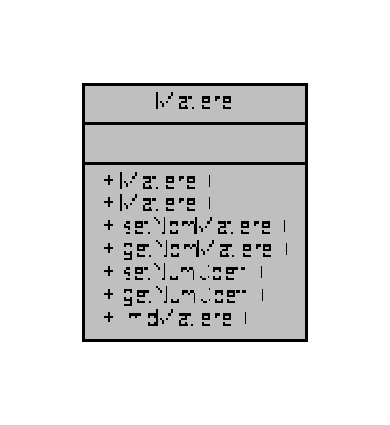
\includegraphics[width=187pt]{class_matiere__coll__graph}
\end{center}
\end{figure}
\subsection*{Public Member Functions}
\begin{DoxyCompactItemize}
\item 
\hyperlink{class_matiere_a0d9dbc35cd0221225366e2ba189c4b42}{Matiere} ()
\item 
\hyperlink{class_matiere_ae70756b9d319ed60372661085615f494}{Matiere} (string la\+Matieres, int le\+Coeff)
\item 
void \hyperlink{class_matiere_af33ccb2e0fa48a8cb25321ba2333791b}{set\+Nom\+Matiere} (string la\+Matiere)
\begin{DoxyCompactList}\small\item\em Initialise la valeur de Nom\+Matiere. \end{DoxyCompactList}\item 
string \hyperlink{class_matiere_a5a31f5b5b20f39cdbf6136cde25ecd31}{get\+Nom\+Matiere} ()
\item 
void \hyperlink{class_matiere_a8890ab57fcdbb6c90c81de7315a38f8b}{set\+Num\+Coeff} (int le\+Coeff)
\begin{DoxyCompactList}\small\item\em initialise la valeur de Num\+Coeff \end{DoxyCompactList}\item 
int \hyperlink{class_matiere_acde1642295616bbcdac2fe270563d12f}{get\+Num\+Coeff} ()
\item 
void \hyperlink{class_matiere_a7f60252430a2517a7c0124d5abe1240e}{info\+Matiere} ()
\begin{DoxyCompactList}\small\item\em saisie d'une matiere et du coeff correspondant Permet à l'utilisateur de saisir une matière et son coefficient correspondant \end{DoxyCompactList}\end{DoxyCompactItemize}


\subsection{Constructor \& Destructor Documentation}
\hypertarget{class_matiere_a0d9dbc35cd0221225366e2ba189c4b42}{\index{Matiere@{Matiere}!Matiere@{Matiere}}
\index{Matiere@{Matiere}!Matiere@{Matiere}}
\subsubsection[{Matiere}]{\setlength{\rightskip}{0pt plus 5cm}Matiere\+::\+Matiere (
\begin{DoxyParamCaption}
{}
\end{DoxyParamCaption}
)}}\label{class_matiere_a0d9dbc35cd0221225366e2ba189c4b42}
Empty constructeur \hypertarget{class_matiere_ae70756b9d319ed60372661085615f494}{\index{Matiere@{Matiere}!Matiere@{Matiere}}
\index{Matiere@{Matiere}!Matiere@{Matiere}}
\subsubsection[{Matiere}]{\setlength{\rightskip}{0pt plus 5cm}Matiere\+::\+Matiere (
\begin{DoxyParamCaption}
\item[{string}]{la\+Matieres, }
\item[{int}]{le\+Coeff}
\end{DoxyParamCaption}
)}}\label{class_matiere_ae70756b9d319ed60372661085615f494}


\subsection{Member Function Documentation}
\hypertarget{class_matiere_a5a31f5b5b20f39cdbf6136cde25ecd31}{\index{Matiere@{Matiere}!get\+Nom\+Matiere@{get\+Nom\+Matiere}}
\index{get\+Nom\+Matiere@{get\+Nom\+Matiere}!Matiere@{Matiere}}
\subsubsection[{get\+Nom\+Matiere}]{\setlength{\rightskip}{0pt plus 5cm}string Matiere\+::get\+Nom\+Matiere (
\begin{DoxyParamCaption}
{}
\end{DoxyParamCaption}
)}}\label{class_matiere_a5a31f5b5b20f39cdbf6136cde25ecd31}
\begin{DoxyReturn}{Returns}
la valeur de Nom\+Matiere
\end{DoxyReturn}
Retourne la valeur de la propriété Nom\+Matiere

Get the value of nom \begin{DoxyReturn}{Returns}
the value of nom 
\end{DoxyReturn}
\hypertarget{class_matiere_acde1642295616bbcdac2fe270563d12f}{\index{Matiere@{Matiere}!get\+Num\+Coeff@{get\+Num\+Coeff}}
\index{get\+Num\+Coeff@{get\+Num\+Coeff}!Matiere@{Matiere}}
\subsubsection[{get\+Num\+Coeff}]{\setlength{\rightskip}{0pt plus 5cm}int Matiere\+::get\+Num\+Coeff (
\begin{DoxyParamCaption}
{}
\end{DoxyParamCaption}
)}}\label{class_matiere_acde1642295616bbcdac2fe270563d12f}
\begin{DoxyReturn}{Returns}
la valeur de Num\+Coeff
\end{DoxyReturn}
Retourne la valeur de la propriété Num\+Coeff \hypertarget{class_matiere_a7f60252430a2517a7c0124d5abe1240e}{\index{Matiere@{Matiere}!info\+Matiere@{info\+Matiere}}
\index{info\+Matiere@{info\+Matiere}!Matiere@{Matiere}}
\subsubsection[{info\+Matiere}]{\setlength{\rightskip}{0pt plus 5cm}void Matiere\+::info\+Matiere (
\begin{DoxyParamCaption}
{}
\end{DoxyParamCaption}
)}}\label{class_matiere_a7f60252430a2517a7c0124d5abe1240e}


saisie d'une matiere et du coeff correspondant Permet à l'utilisateur de saisir une matière et son coefficient correspondant 

\hypertarget{class_matiere_af33ccb2e0fa48a8cb25321ba2333791b}{\index{Matiere@{Matiere}!set\+Nom\+Matiere@{set\+Nom\+Matiere}}
\index{set\+Nom\+Matiere@{set\+Nom\+Matiere}!Matiere@{Matiere}}
\subsubsection[{set\+Nom\+Matiere}]{\setlength{\rightskip}{0pt plus 5cm}void Matiere\+::set\+Nom\+Matiere (
\begin{DoxyParamCaption}
\item[{string}]{la\+Matiere}
\end{DoxyParamCaption}
)}}\label{class_matiere_af33ccb2e0fa48a8cb25321ba2333791b}


Initialise la valeur de Nom\+Matiere. 


\begin{DoxyParams}{Parameters}
{\em la\+Matiere} & reçoit Nom\+Matiere\\
\hline
\end{DoxyParams}
donne le nom de la matiere 
\begin{DoxyParams}{Parameters}
{\em la\+Matiere} & la nouvelle valeur de nom\+Matiere \\
\hline
\end{DoxyParams}
\hypertarget{class_matiere_a8890ab57fcdbb6c90c81de7315a38f8b}{\index{Matiere@{Matiere}!set\+Num\+Coeff@{set\+Num\+Coeff}}
\index{set\+Num\+Coeff@{set\+Num\+Coeff}!Matiere@{Matiere}}
\subsubsection[{set\+Num\+Coeff}]{\setlength{\rightskip}{0pt plus 5cm}void Matiere\+::set\+Num\+Coeff (
\begin{DoxyParamCaption}
\item[{int}]{le\+Coeff}
\end{DoxyParamCaption}
)}}\label{class_matiere_a8890ab57fcdbb6c90c81de7315a38f8b}


initialise la valeur de Num\+Coeff 


\begin{DoxyParams}{Parameters}
{\em le\+Coeff} & reçoit Num\+Coeff \\
\hline
\end{DoxyParams}


The documentation for this class was generated from the following files\+:\begin{DoxyCompactItemize}
\item 
\hyperlink{_matiere_8h}{Matiere.\+h}\item 
\hyperlink{_matiere_8cpp}{Matiere.\+cpp}\end{DoxyCompactItemize}

\hypertarget{class_notes}{\section{Notes Class Reference}
\label{class_notes}\index{Notes@{Notes}}
}


{\ttfamily \#include $<$Notes.\+h$>$}



Collaboration diagram for Notes\+:\nopagebreak
\begin{figure}[H]
\begin{center}
\leavevmode
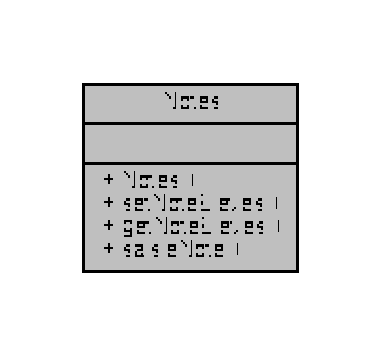
\includegraphics[width=183pt]{class_notes__coll__graph}
\end{center}
\end{figure}
\subsection*{Public Member Functions}
\begin{DoxyCompactItemize}
\item 
\hyperlink{class_notes_ad031ee5187c64b36036a1486c2ec5d0b}{Notes} ()
\item 
void \hyperlink{class_notes_a7e1ffa4316f63d07e14c74542cdaf9bf}{set\+Note\+Eleves} (float la\+Note)
\begin{DoxyCompactList}\small\item\em Initialiser la valeur de Note\+Eleves. \end{DoxyCompactList}\item 
float \hyperlink{class_notes_a122f1318b07dd9155ab83d08dbc6708f}{get\+Note\+Eleves} ()
\item 
void \hyperlink{class_notes_a294991e8d30e40537a35803d64b655d3}{saisie\+Note} ()
\begin{DoxyCompactList}\small\item\em saisie note Permet à l'utilisateur de saisir la valeur d'une note \end{DoxyCompactList}\end{DoxyCompactItemize}


\subsection{Constructor \& Destructor Documentation}
\hypertarget{class_notes_ad031ee5187c64b36036a1486c2ec5d0b}{\index{Notes@{Notes}!Notes@{Notes}}
\index{Notes@{Notes}!Notes@{Notes}}
\subsubsection[{Notes}]{\setlength{\rightskip}{0pt plus 5cm}Notes\+::\+Notes (
\begin{DoxyParamCaption}
{}
\end{DoxyParamCaption}
)}}\label{class_notes_ad031ee5187c64b36036a1486c2ec5d0b}
Empty Constructor 

\subsection{Member Function Documentation}
\hypertarget{class_notes_a122f1318b07dd9155ab83d08dbc6708f}{\index{Notes@{Notes}!get\+Note\+Eleves@{get\+Note\+Eleves}}
\index{get\+Note\+Eleves@{get\+Note\+Eleves}!Notes@{Notes}}
\subsubsection[{get\+Note\+Eleves}]{\setlength{\rightskip}{0pt plus 5cm}float Notes\+::get\+Note\+Eleves (
\begin{DoxyParamCaption}
{}
\end{DoxyParamCaption}
)}}\label{class_notes_a122f1318b07dd9155ab83d08dbc6708f}
\begin{DoxyReturn}{Returns}
la valeur de Note\+Eleves
\end{DoxyReturn}
Retourne la valeur de la propriété Note\+Eleves

Get the value of note \begin{DoxyReturn}{Returns}
the value of note 
\end{DoxyReturn}
\hypertarget{class_notes_a294991e8d30e40537a35803d64b655d3}{\index{Notes@{Notes}!saisie\+Note@{saisie\+Note}}
\index{saisie\+Note@{saisie\+Note}!Notes@{Notes}}
\subsubsection[{saisie\+Note}]{\setlength{\rightskip}{0pt plus 5cm}void Notes\+::saisie\+Note (
\begin{DoxyParamCaption}
{}
\end{DoxyParamCaption}
)}}\label{class_notes_a294991e8d30e40537a35803d64b655d3}


saisie note Permet à l'utilisateur de saisir la valeur d'une note 

Set the value of proprietaire 
\begin{DoxyParams}{Parameters}
{\em new\+\_\+var} & the new value of proprietaire Get the value of proprietaire \\
\hline
\end{DoxyParams}
\begin{DoxyReturn}{Returns}
the value of proprietaire 
\end{DoxyReturn}
\hypertarget{class_notes_a7e1ffa4316f63d07e14c74542cdaf9bf}{\index{Notes@{Notes}!set\+Note\+Eleves@{set\+Note\+Eleves}}
\index{set\+Note\+Eleves@{set\+Note\+Eleves}!Notes@{Notes}}
\subsubsection[{set\+Note\+Eleves}]{\setlength{\rightskip}{0pt plus 5cm}void Notes\+::set\+Note\+Eleves (
\begin{DoxyParamCaption}
\item[{float}]{la\+Note}
\end{DoxyParamCaption}
)}}\label{class_notes_a7e1ffa4316f63d07e14c74542cdaf9bf}


Initialiser la valeur de Note\+Eleves. 


\begin{DoxyParams}{Parameters}
{\em la\+Note} & reçoit comme valeur Note\+Eleves\\
\hline
\end{DoxyParams}
Set the value of note 
\begin{DoxyParams}{Parameters}
{\em new\+\_\+var} & the new value of note \\
\hline
\end{DoxyParams}


The documentation for this class was generated from the following files\+:\begin{DoxyCompactItemize}
\item 
\hyperlink{_notes_8h}{Notes.\+h}\item 
\hyperlink{_notes_8cpp}{Notes.\+cpp}\end{DoxyCompactItemize}

\hypertarget{class_section}{\section{Section Class Reference}
\label{class_section}\index{Section@{Section}}
}


{\ttfamily \#include $<$Section.\+h$>$}



Collaboration diagram for Section\+:\nopagebreak
\begin{figure}[H]
\begin{center}
\leavevmode
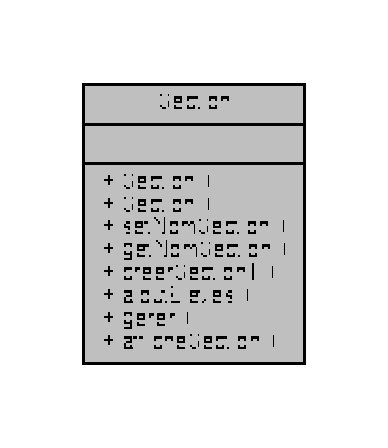
\includegraphics[width=186pt]{class_section__coll__graph}
\end{center}
\end{figure}
\subsection*{Public Member Functions}
\begin{DoxyCompactItemize}
\item 
\hyperlink{class_section_a77b88e06692841ba49559d22a25a09f9}{Section} ()
\item 
\hyperlink{class_section_acc03e01cbc50c87d37e02b4168d6e0fc}{Section} (string la\+Sections)
\item 
void \hyperlink{class_section_adc7f73c7e76c73de88d8c59170a67383}{set\+Nom\+Section} (string la\+Section)
\begin{DoxyCompactList}\small\item\em Initialise la valeur de Nom\+Section. \end{DoxyCompactList}\item 
string \hyperlink{class_section_a432b7a6163aa6225e74de5560fe09b00}{get\+Nom\+Section} ()
\item 
void \hyperlink{class_section_a6d5c8df796b9a0664319bd768983225e}{creer\+Section1} ()
\begin{DoxyCompactList}\small\item\em création d'une section Permet à l'utilisateur de saisir les valeur de la section afin de la créer \end{DoxyCompactList}\item 
void \hyperlink{class_section_aa032f59ebbe6ade8bfb9a88eb1bf9240}{ajout\+Eleves} ()
\begin{DoxyCompactList}\small\item\em ajout d'un élève dans une section Permet à l'utilisateur d'ajouter les valeurs de l'élève dans la section sélectionné \end{DoxyCompactList}\item 
void \hyperlink{class_section_a0c869f228298503305cf7be8e8e3df91}{gerer} ()
\begin{DoxyCompactList}\small\item\em gérer une section Permet à l'utilisateur de gérer la section choisie, il a le choix entre\+: ajouter un élève, consulter les élèves présents dans la section, et ajouter une matière \end{DoxyCompactList}\item 
void \hyperlink{class_section_a68d0635c31799fcaa45d6629653296de}{affiche\+Section} ()
\begin{DoxyCompactList}\small\item\em Affiche les élèves présent dans la section précisée Permet à l'utilisateur d'afficher dans la section choisie qui est précisée, les élèves présent dans la section. \end{DoxyCompactList}\end{DoxyCompactItemize}


\subsection{Constructor \& Destructor Documentation}
\hypertarget{class_section_a77b88e06692841ba49559d22a25a09f9}{\index{Section@{Section}!Section@{Section}}
\index{Section@{Section}!Section@{Section}}
\subsubsection[{Section}]{\setlength{\rightskip}{0pt plus 5cm}Section\+::\+Section (
\begin{DoxyParamCaption}
{}
\end{DoxyParamCaption}
)}}\label{class_section_a77b88e06692841ba49559d22a25a09f9}
Empty Constructor \hypertarget{class_section_acc03e01cbc50c87d37e02b4168d6e0fc}{\index{Section@{Section}!Section@{Section}}
\index{Section@{Section}!Section@{Section}}
\subsubsection[{Section}]{\setlength{\rightskip}{0pt plus 5cm}Section\+::\+Section (
\begin{DoxyParamCaption}
\item[{string}]{la\+Sections}
\end{DoxyParamCaption}
)}}\label{class_section_acc03e01cbc50c87d37e02b4168d6e0fc}


\subsection{Member Function Documentation}
\hypertarget{class_section_a68d0635c31799fcaa45d6629653296de}{\index{Section@{Section}!affiche\+Section@{affiche\+Section}}
\index{affiche\+Section@{affiche\+Section}!Section@{Section}}
\subsubsection[{affiche\+Section}]{\setlength{\rightskip}{0pt plus 5cm}void Section\+::affiche\+Section (
\begin{DoxyParamCaption}
{}
\end{DoxyParamCaption}
)}}\label{class_section_a68d0635c31799fcaa45d6629653296de}


Affiche les élèves présent dans la section précisée Permet à l'utilisateur d'afficher dans la section choisie qui est précisée, les élèves présent dans la section. 



Here is the caller graph for this function\+:\nopagebreak
\begin{figure}[H]
\begin{center}
\leavevmode
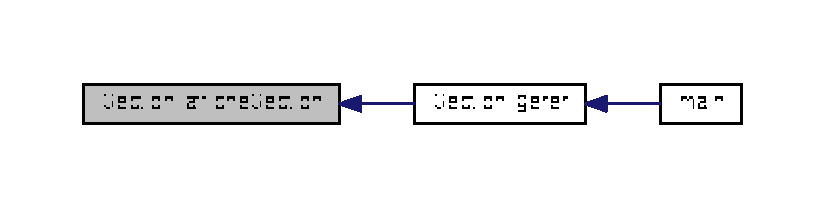
\includegraphics[width=350pt]{class_section_a68d0635c31799fcaa45d6629653296de_icgraph}
\end{center}
\end{figure}


\hypertarget{class_section_aa032f59ebbe6ade8bfb9a88eb1bf9240}{\index{Section@{Section}!ajout\+Eleves@{ajout\+Eleves}}
\index{ajout\+Eleves@{ajout\+Eleves}!Section@{Section}}
\subsubsection[{ajout\+Eleves}]{\setlength{\rightskip}{0pt plus 5cm}void Section\+::ajout\+Eleves (
\begin{DoxyParamCaption}
{}
\end{DoxyParamCaption}
)}}\label{class_section_aa032f59ebbe6ade8bfb9a88eb1bf9240}


ajout d'un élève dans une section Permet à l'utilisateur d'ajouter les valeurs de l'élève dans la section sélectionné 



Here is the call graph for this function\+:\nopagebreak
\begin{figure}[H]
\begin{center}
\leavevmode
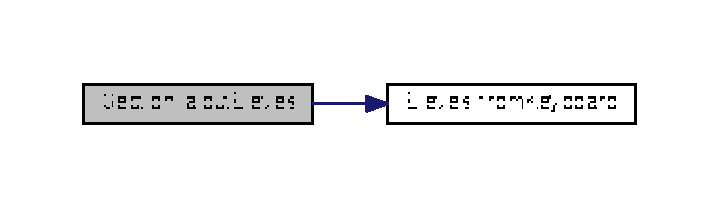
\includegraphics[width=345pt]{class_section_aa032f59ebbe6ade8bfb9a88eb1bf9240_cgraph}
\end{center}
\end{figure}




Here is the caller graph for this function\+:\nopagebreak
\begin{figure}[H]
\begin{center}
\leavevmode
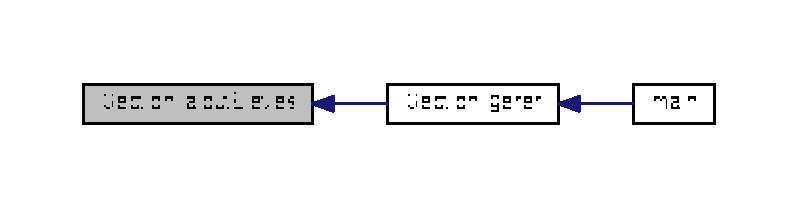
\includegraphics[width=350pt]{class_section_aa032f59ebbe6ade8bfb9a88eb1bf9240_icgraph}
\end{center}
\end{figure}


\hypertarget{class_section_a6d5c8df796b9a0664319bd768983225e}{\index{Section@{Section}!creer\+Section1@{creer\+Section1}}
\index{creer\+Section1@{creer\+Section1}!Section@{Section}}
\subsubsection[{creer\+Section1}]{\setlength{\rightskip}{0pt plus 5cm}void Section\+::creer\+Section1 (
\begin{DoxyParamCaption}
{}
\end{DoxyParamCaption}
)}}\label{class_section_a6d5c8df796b9a0664319bd768983225e}


création d'une section Permet à l'utilisateur de saisir les valeur de la section afin de la créer 

\hypertarget{class_section_a0c869f228298503305cf7be8e8e3df91}{\index{Section@{Section}!gerer@{gerer}}
\index{gerer@{gerer}!Section@{Section}}
\subsubsection[{gerer}]{\setlength{\rightskip}{0pt plus 5cm}void Section\+::gerer (
\begin{DoxyParamCaption}
{}
\end{DoxyParamCaption}
)}}\label{class_section_a0c869f228298503305cf7be8e8e3df91}


gérer une section Permet à l'utilisateur de gérer la section choisie, il a le choix entre\+: ajouter un élève, consulter les élèves présents dans la section, et ajouter une matière 



Here is the call graph for this function\+:\nopagebreak
\begin{figure}[H]
\begin{center}
\leavevmode
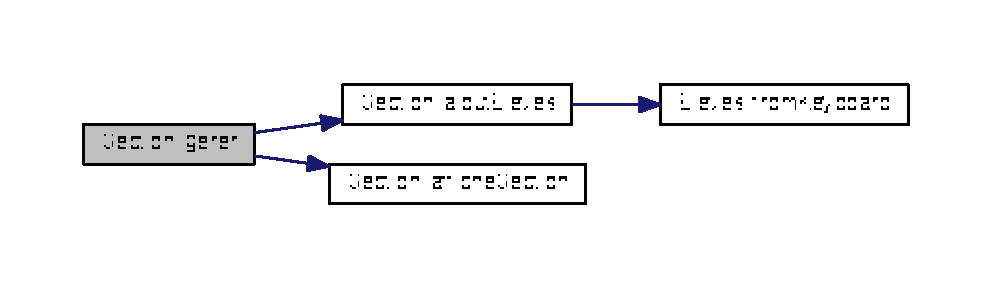
\includegraphics[width=350pt]{class_section_a0c869f228298503305cf7be8e8e3df91_cgraph}
\end{center}
\end{figure}




Here is the caller graph for this function\+:\nopagebreak
\begin{figure}[H]
\begin{center}
\leavevmode
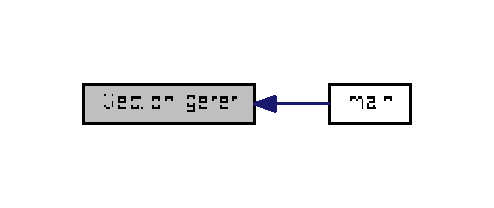
\includegraphics[width=237pt]{class_section_a0c869f228298503305cf7be8e8e3df91_icgraph}
\end{center}
\end{figure}


\hypertarget{class_section_a432b7a6163aa6225e74de5560fe09b00}{\index{Section@{Section}!get\+Nom\+Section@{get\+Nom\+Section}}
\index{get\+Nom\+Section@{get\+Nom\+Section}!Section@{Section}}
\subsubsection[{get\+Nom\+Section}]{\setlength{\rightskip}{0pt plus 5cm}string Section\+::get\+Nom\+Section (
\begin{DoxyParamCaption}
{}
\end{DoxyParamCaption}
)}}\label{class_section_a432b7a6163aa6225e74de5560fe09b00}
\begin{DoxyReturn}{Returns}
la valeur de Nom\+Section
\end{DoxyReturn}
Retourne la valeur de la propriété Nom\+Section

Get the value of nom \begin{DoxyReturn}{Returns}
the value of nom 
\end{DoxyReturn}
\hypertarget{class_section_adc7f73c7e76c73de88d8c59170a67383}{\index{Section@{Section}!set\+Nom\+Section@{set\+Nom\+Section}}
\index{set\+Nom\+Section@{set\+Nom\+Section}!Section@{Section}}
\subsubsection[{set\+Nom\+Section}]{\setlength{\rightskip}{0pt plus 5cm}void Section\+::set\+Nom\+Section (
\begin{DoxyParamCaption}
\item[{string}]{la\+Section}
\end{DoxyParamCaption}
)}}\label{class_section_adc7f73c7e76c73de88d8c59170a67383}


Initialise la valeur de Nom\+Section. 


\begin{DoxyParams}{Parameters}
{\em la\+Section} & reçoit Nom\+Section\\
\hline
\end{DoxyParams}
Set the value of nom 
\begin{DoxyParams}{Parameters}
{\em new\+\_\+var} & the new value of nom \\
\hline
\end{DoxyParams}


Here is the caller graph for this function\+:\nopagebreak
\begin{figure}[H]
\begin{center}
\leavevmode
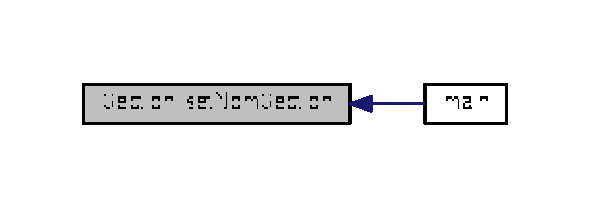
\includegraphics[width=283pt]{class_section_adc7f73c7e76c73de88d8c59170a67383_icgraph}
\end{center}
\end{figure}




The documentation for this class was generated from the following files\+:\begin{DoxyCompactItemize}
\item 
\hyperlink{_section_8h}{Section.\+h}\item 
\hyperlink{_section_8cpp}{Section.\+cpp}\end{DoxyCompactItemize}

\chapter{File Documentation}
\hypertarget{eleves_8cpp}{\section{eleves.\+cpp File Reference}
\label{eleves_8cpp}\index{eleves.\+cpp@{eleves.\+cpp}}
}
{\ttfamily \#include \char`\"{}eleves.\+h\char`\"{}}\\*
{\ttfamily \#include $<$iostream$>$}\\*
Include dependency graph for eleves.\+cpp\+:\nopagebreak
\begin{figure}[H]
\begin{center}
\leavevmode
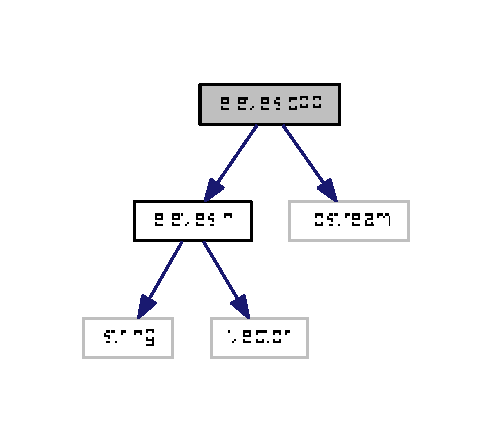
\includegraphics[width=236pt]{eleves_8cpp__incl}
\end{center}
\end{figure}

\hypertarget{eleves_8h}{\section{eleves.\+h File Reference}
\label{eleves_8h}\index{eleves.\+h@{eleves.\+h}}
}
{\ttfamily \#include $<$string$>$}\\*
{\ttfamily \#include $<$vector$>$}\\*
Include dependency graph for eleves.\+h\+:\nopagebreak
\begin{figure}[H]
\begin{center}
\leavevmode
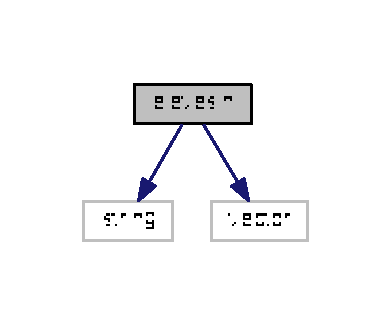
\includegraphics[width=187pt]{eleves_8h__incl}
\end{center}
\end{figure}
This graph shows which files directly or indirectly include this file\+:\nopagebreak
\begin{figure}[H]
\begin{center}
\leavevmode
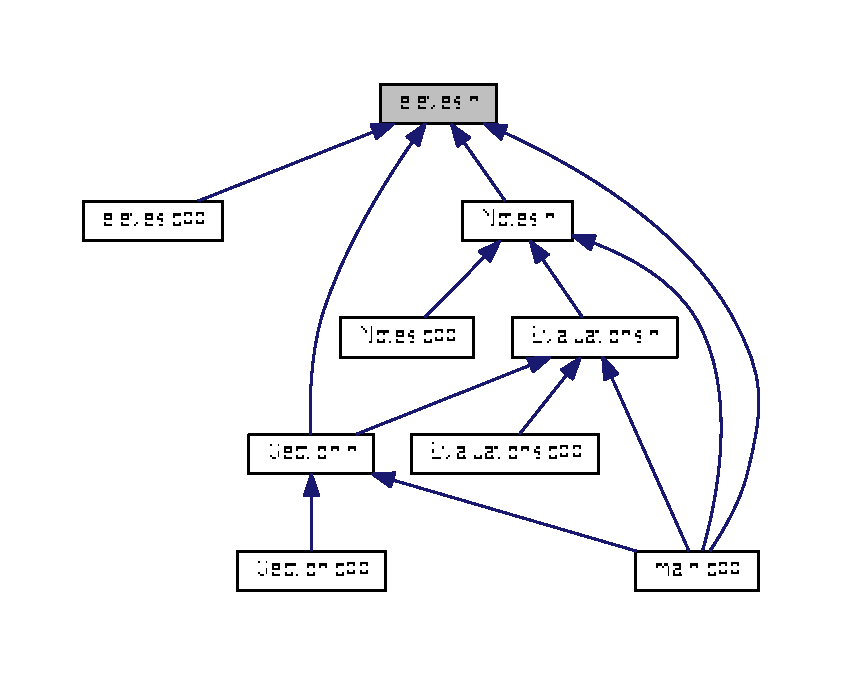
\includegraphics[width=350pt]{eleves_8h__dep__incl}
\end{center}
\end{figure}
\subsection*{Classes}
\begin{DoxyCompactItemize}
\item 
class \hyperlink{class_eleves}{Eleves}
\end{DoxyCompactItemize}

\hypertarget{_evaluations_8cpp}{\section{Evaluations.\+cpp File Reference}
\label{_evaluations_8cpp}\index{Evaluations.\+cpp@{Evaluations.\+cpp}}
}
{\ttfamily \#include \char`\"{}Evaluations.\+h\char`\"{}}\\*
{\ttfamily \#include $<$iostream$>$}\\*
Include dependency graph for Evaluations.\+cpp\+:\nopagebreak
\begin{figure}[H]
\begin{center}
\leavevmode
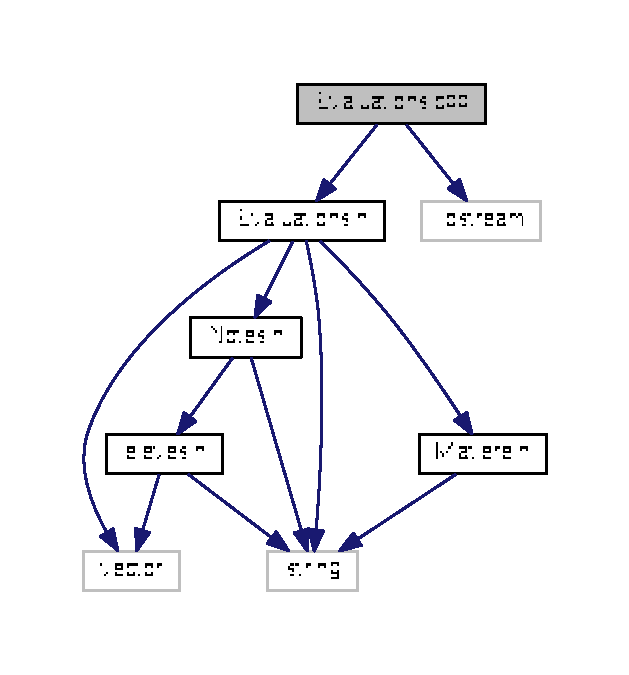
\includegraphics[width=302pt]{_evaluations_8cpp__incl}
\end{center}
\end{figure}

\hypertarget{_evaluations_8h}{\section{Evaluations.\+h File Reference}
\label{_evaluations_8h}\index{Evaluations.\+h@{Evaluations.\+h}}
}
{\ttfamily \#include $<$string$>$}\\*
{\ttfamily \#include $<$vector$>$}\\*
{\ttfamily \#include \char`\"{}Matiere.\+h\char`\"{}}\\*
{\ttfamily \#include \char`\"{}Notes.\+h\char`\"{}}\\*
Include dependency graph for Evaluations.\+h\+:\nopagebreak
\begin{figure}[H]
\begin{center}
\leavevmode
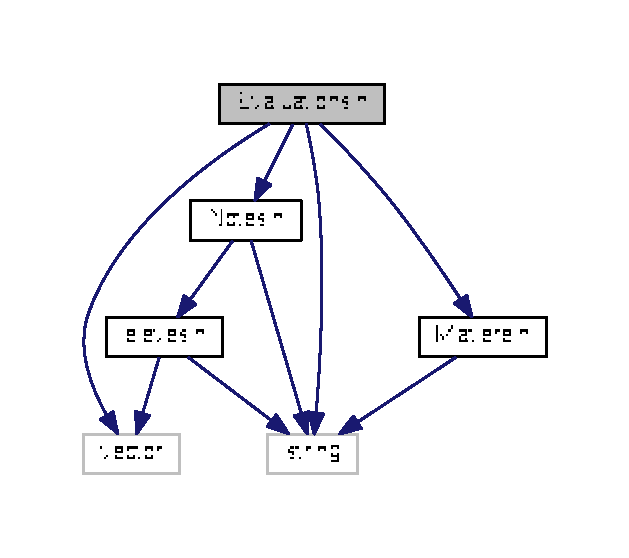
\includegraphics[width=302pt]{_evaluations_8h__incl}
\end{center}
\end{figure}
This graph shows which files directly or indirectly include this file\+:\nopagebreak
\begin{figure}[H]
\begin{center}
\leavevmode
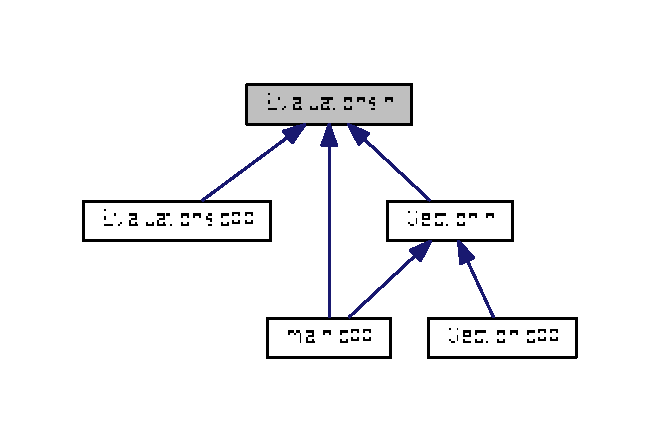
\includegraphics[width=316pt]{_evaluations_8h__dep__incl}
\end{center}
\end{figure}
\subsection*{Classes}
\begin{DoxyCompactItemize}
\item 
class \hyperlink{class_evaluations}{Evaluations}
\end{DoxyCompactItemize}

\hypertarget{main_8cpp}{\section{main.\+cpp File Reference}
\label{main_8cpp}\index{main.\+cpp@{main.\+cpp}}
}
{\ttfamily \#include $<$string$>$}\\*
{\ttfamily \#include $<$iostream$>$}\\*
{\ttfamily \#include $<$vector$>$}\\*
{\ttfamily \#include \char`\"{}eleves.\+h\char`\"{}}\\*
{\ttfamily \#include \char`\"{}Matiere.\+h\char`\"{}}\\*
{\ttfamily \#include \char`\"{}Notes.\+h\char`\"{}}\\*
{\ttfamily \#include \char`\"{}Section.\+h\char`\"{}}\\*
{\ttfamily \#include \char`\"{}Evaluations.\+h\char`\"{}}\\*
Include dependency graph for main.\+cpp\+:\nopagebreak
\begin{figure}[H]
\begin{center}
\leavevmode
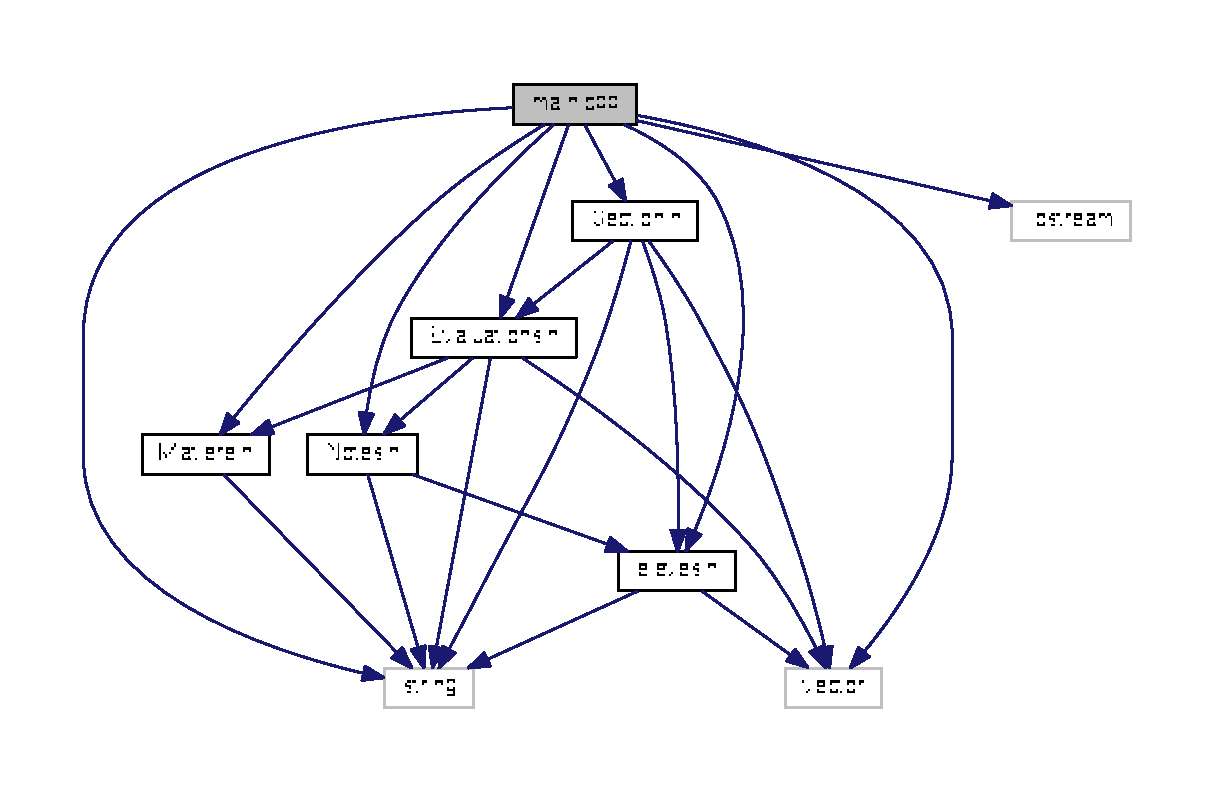
\includegraphics[width=350pt]{main_8cpp__incl}
\end{center}
\end{figure}
\subsection*{Functions}
\begin{DoxyCompactItemize}
\item 
void \hyperlink{main_8cpp_a3f7c5d1e906b11a9eeb8bec6f4b36a10}{affiche\+Section} (vector$<$ \hyperlink{class_section}{Section} $>$ \&le\+Vecteur)
\begin{DoxyCompactList}\small\item\em Affiche la liste des sections Permet d'afficher les sections créées a l'utilisateur. \end{DoxyCompactList}\item 
\hyperlink{class_section}{Section} $\ast$ \hyperlink{main_8cpp_ab4da989a5a85c62e58b2aaaa560d541c}{section\+Selector} (vector$<$ \hyperlink{class_section}{Section} $>$ \&le\+Vecteur)
\begin{DoxyCompactList}\small\item\em Sélection de la section Permet à l'utilisateur de choisir la section désirée à l'aide d'un numéro. \end{DoxyCompactList}\item 
int \hyperlink{main_8cpp_ae66f6b31b5ad750f1fe042a706a4e3d4}{main} ()
\end{DoxyCompactItemize}
\subsection*{Variables}
\begin{DoxyCompactItemize}
\item 
vector$<$ \hyperlink{class_section}{Section} $>$ \hyperlink{main_8cpp_a413e97ee350888cda4f7b6a1f2579249}{vect\+Sections}
\item 
vector$<$ \hyperlink{class_matiere}{Matiere} $>$ \hyperlink{main_8cpp_ac04b2ba8d7488df23bc7f9122d15434d}{vect\+Mat}
\item 
vector$<$ \hyperlink{class_evaluations}{Evaluations} $>$ \hyperlink{main_8cpp_aa8b35d7b93c19ac3a2cdc1900eac6c21}{vect\+Eval}
\item 
vector$<$ \hyperlink{class_eleves}{Eleves} $>$ \hyperlink{main_8cpp_a892cd6fca64a12f2ea86dced68c1b8fa}{vect\+Eleves}
\end{DoxyCompactItemize}


\subsection{Function Documentation}
\hypertarget{main_8cpp_a3f7c5d1e906b11a9eeb8bec6f4b36a10}{\index{main.\+cpp@{main.\+cpp}!affiche\+Section@{affiche\+Section}}
\index{affiche\+Section@{affiche\+Section}!main.\+cpp@{main.\+cpp}}
\subsubsection[{affiche\+Section}]{\setlength{\rightskip}{0pt plus 5cm}void affiche\+Section (
\begin{DoxyParamCaption}
\item[{vector$<$ {\bf Section} $>$ \&}]{le\+Vecteur}
\end{DoxyParamCaption}
)}}\label{main_8cpp_a3f7c5d1e906b11a9eeb8bec6f4b36a10}


Affiche la liste des sections Permet d'afficher les sections créées a l'utilisateur. 


\begin{DoxyParams}{Parameters}
{\em le\+Vecteur} & reçoit nb\+Section \\
\hline
\end{DoxyParams}


Here is the caller graph for this function\+:
\nopagebreak
\begin{figure}[H]
\begin{center}
\leavevmode
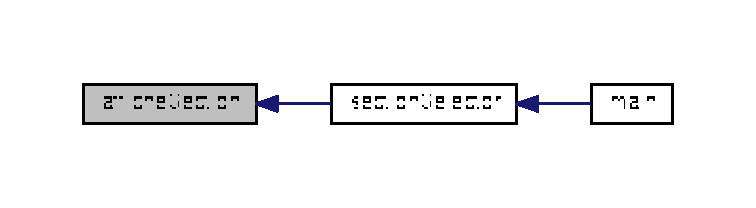
\includegraphics[width=350pt]{main_8cpp_a3f7c5d1e906b11a9eeb8bec6f4b36a10_icgraph}
\end{center}
\end{figure}


\hypertarget{main_8cpp_ae66f6b31b5ad750f1fe042a706a4e3d4}{\index{main.\+cpp@{main.\+cpp}!main@{main}}
\index{main@{main}!main.\+cpp@{main.\+cpp}}
\subsubsection[{main}]{\setlength{\rightskip}{0pt plus 5cm}int main (
\begin{DoxyParamCaption}
{}
\end{DoxyParamCaption}
)}}\label{main_8cpp_ae66f6b31b5ad750f1fe042a706a4e3d4}


Here is the call graph for this function\+:
\nopagebreak
\begin{figure}[H]
\begin{center}
\leavevmode
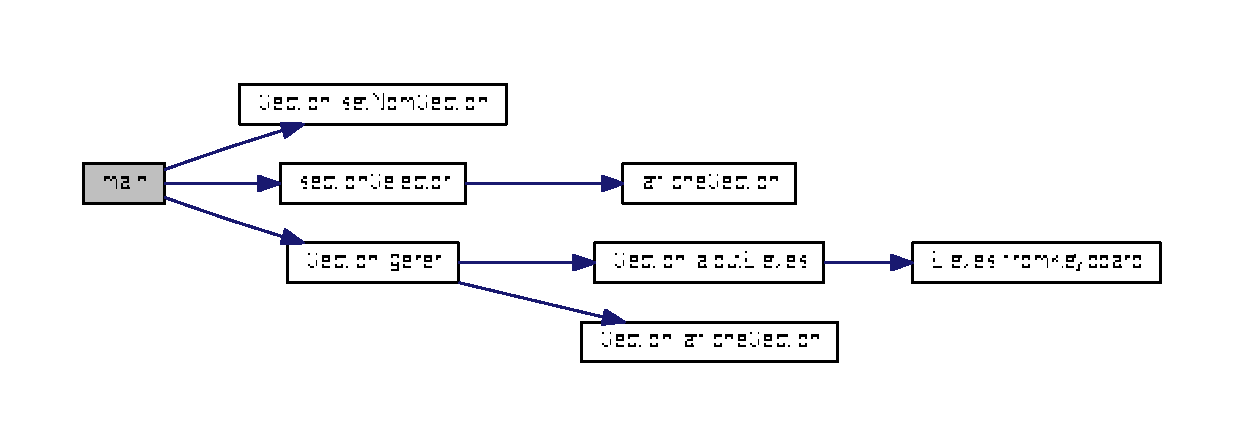
\includegraphics[width=350pt]{main_8cpp_ae66f6b31b5ad750f1fe042a706a4e3d4_cgraph}
\end{center}
\end{figure}


\hypertarget{main_8cpp_ab4da989a5a85c62e58b2aaaa560d541c}{\index{main.\+cpp@{main.\+cpp}!section\+Selector@{section\+Selector}}
\index{section\+Selector@{section\+Selector}!main.\+cpp@{main.\+cpp}}
\subsubsection[{section\+Selector}]{\setlength{\rightskip}{0pt plus 5cm}{\bf Section}$\ast$ section\+Selector (
\begin{DoxyParamCaption}
\item[{vector$<$ {\bf Section} $>$ \&}]{le\+Vecteur}
\end{DoxyParamCaption}
)}}\label{main_8cpp_ab4da989a5a85c62e58b2aaaa560d541c}


Sélection de la section Permet à l'utilisateur de choisir la section désirée à l'aide d'un numéro. 


\begin{DoxyParams}{Parameters}
{\em le\+Vecteur} & reçoit nb\+Section \\
\hline
\end{DoxyParams}
\begin{DoxyReturn}{Returns}
la valeur de le\+Vecteur 
\end{DoxyReturn}


Here is the call graph for this function\+:
\nopagebreak
\begin{figure}[H]
\begin{center}
\leavevmode
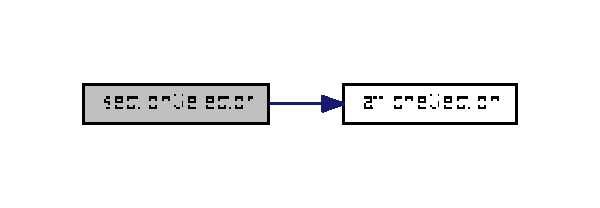
\includegraphics[width=288pt]{main_8cpp_ab4da989a5a85c62e58b2aaaa560d541c_cgraph}
\end{center}
\end{figure}




Here is the caller graph for this function\+:\nopagebreak
\begin{figure}[H]
\begin{center}
\leavevmode
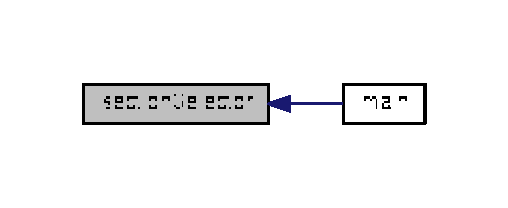
\includegraphics[width=244pt]{main_8cpp_ab4da989a5a85c62e58b2aaaa560d541c_icgraph}
\end{center}
\end{figure}




\subsection{Variable Documentation}
\hypertarget{main_8cpp_a892cd6fca64a12f2ea86dced68c1b8fa}{\index{main.\+cpp@{main.\+cpp}!vect\+Eleves@{vect\+Eleves}}
\index{vect\+Eleves@{vect\+Eleves}!main.\+cpp@{main.\+cpp}}
\subsubsection[{vect\+Eleves}]{\setlength{\rightskip}{0pt plus 5cm}vector$<${\bf Eleves}$>$ vect\+Eleves}}\label{main_8cpp_a892cd6fca64a12f2ea86dced68c1b8fa}
\hypertarget{main_8cpp_aa8b35d7b93c19ac3a2cdc1900eac6c21}{\index{main.\+cpp@{main.\+cpp}!vect\+Eval@{vect\+Eval}}
\index{vect\+Eval@{vect\+Eval}!main.\+cpp@{main.\+cpp}}
\subsubsection[{vect\+Eval}]{\setlength{\rightskip}{0pt plus 5cm}vector$<${\bf Evaluations}$>$ vect\+Eval}}\label{main_8cpp_aa8b35d7b93c19ac3a2cdc1900eac6c21}
\hypertarget{main_8cpp_ac04b2ba8d7488df23bc7f9122d15434d}{\index{main.\+cpp@{main.\+cpp}!vect\+Mat@{vect\+Mat}}
\index{vect\+Mat@{vect\+Mat}!main.\+cpp@{main.\+cpp}}
\subsubsection[{vect\+Mat}]{\setlength{\rightskip}{0pt plus 5cm}vector$<${\bf Matiere}$>$ vect\+Mat}}\label{main_8cpp_ac04b2ba8d7488df23bc7f9122d15434d}
\hypertarget{main_8cpp_a413e97ee350888cda4f7b6a1f2579249}{\index{main.\+cpp@{main.\+cpp}!vect\+Sections@{vect\+Sections}}
\index{vect\+Sections@{vect\+Sections}!main.\+cpp@{main.\+cpp}}
\subsubsection[{vect\+Sections}]{\setlength{\rightskip}{0pt plus 5cm}vector$<${\bf Section}$>$ vect\+Sections}}\label{main_8cpp_a413e97ee350888cda4f7b6a1f2579249}

\hypertarget{_matiere_8cpp}{\section{Matiere.\+cpp File Reference}
\label{_matiere_8cpp}\index{Matiere.\+cpp@{Matiere.\+cpp}}
}
{\ttfamily \#include \char`\"{}Matiere.\+h\char`\"{}}\\*
{\ttfamily \#include $<$iostream$>$}\\*
Include dependency graph for Matiere.\+cpp\+:\nopagebreak
\begin{figure}[H]
\begin{center}
\leavevmode
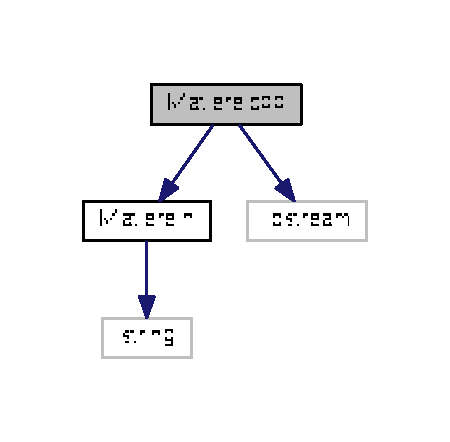
\includegraphics[width=216pt]{_matiere_8cpp__incl}
\end{center}
\end{figure}

\hypertarget{_matiere_8h}{\section{Matiere.\+h File Reference}
\label{_matiere_8h}\index{Matiere.\+h@{Matiere.\+h}}
}
{\ttfamily \#include $<$string$>$}\\*
Include dependency graph for Matiere.\+h\+:\nopagebreak
\begin{figure}[H]
\begin{center}
\leavevmode
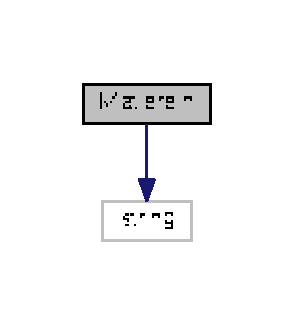
\includegraphics[width=141pt]{_matiere_8h__incl}
\end{center}
\end{figure}
This graph shows which files directly or indirectly include this file\+:\nopagebreak
\begin{figure}[H]
\begin{center}
\leavevmode
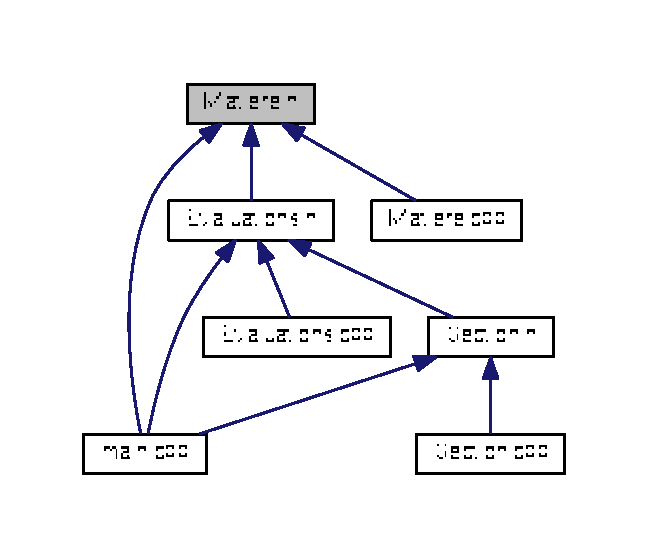
\includegraphics[width=311pt]{_matiere_8h__dep__incl}
\end{center}
\end{figure}
\subsection*{Classes}
\begin{DoxyCompactItemize}
\item 
class \hyperlink{class_matiere}{Matiere}
\end{DoxyCompactItemize}

\hypertarget{_notes_8cpp}{\section{Notes.\+cpp File Reference}
\label{_notes_8cpp}\index{Notes.\+cpp@{Notes.\+cpp}}
}
{\ttfamily \#include \char`\"{}Notes.\+h\char`\"{}}\\*
{\ttfamily \#include $<$iostream$>$}\\*
Include dependency graph for Notes.\+cpp\+:\nopagebreak
\begin{figure}[H]
\begin{center}
\leavevmode
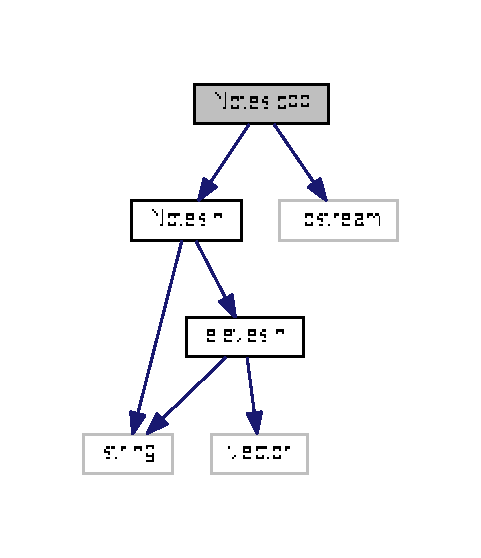
\includegraphics[width=231pt]{_notes_8cpp__incl}
\end{center}
\end{figure}

\hypertarget{_notes_8h}{\section{Notes.\+h File Reference}
\label{_notes_8h}\index{Notes.\+h@{Notes.\+h}}
}
{\ttfamily \#include $<$string$>$}\\*
{\ttfamily \#include \char`\"{}eleves.\+h\char`\"{}}\\*
Include dependency graph for Notes.\+h\+:\nopagebreak
\begin{figure}[H]
\begin{center}
\leavevmode
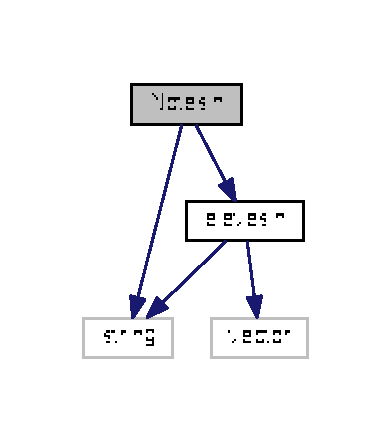
\includegraphics[width=187pt]{_notes_8h__incl}
\end{center}
\end{figure}
This graph shows which files directly or indirectly include this file\+:\nopagebreak
\begin{figure}[H]
\begin{center}
\leavevmode
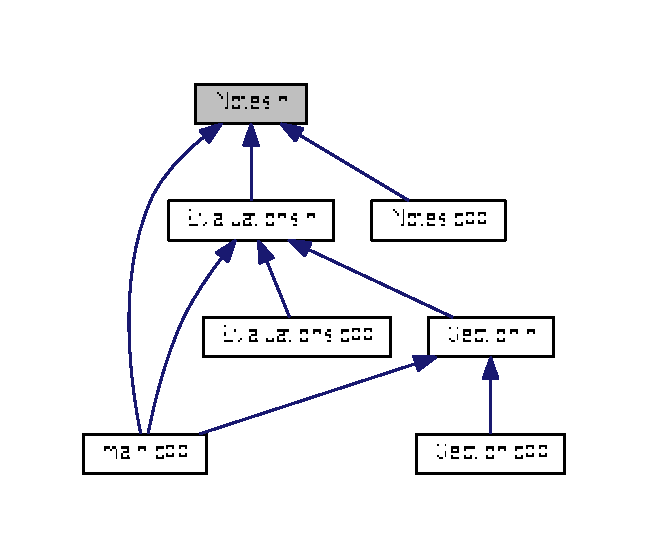
\includegraphics[width=311pt]{_notes_8h__dep__incl}
\end{center}
\end{figure}
\subsection*{Classes}
\begin{DoxyCompactItemize}
\item 
class \hyperlink{class_notes}{Notes}
\end{DoxyCompactItemize}

\hypertarget{_section_8cpp}{\section{Section.\+cpp File Reference}
\label{_section_8cpp}\index{Section.\+cpp@{Section.\+cpp}}
}
{\ttfamily \#include \char`\"{}Section.\+h\char`\"{}}\\*
{\ttfamily \#include $<$iostream$>$}\\*
Include dependency graph for Section.\+cpp\+:\nopagebreak
\begin{figure}[H]
\begin{center}
\leavevmode
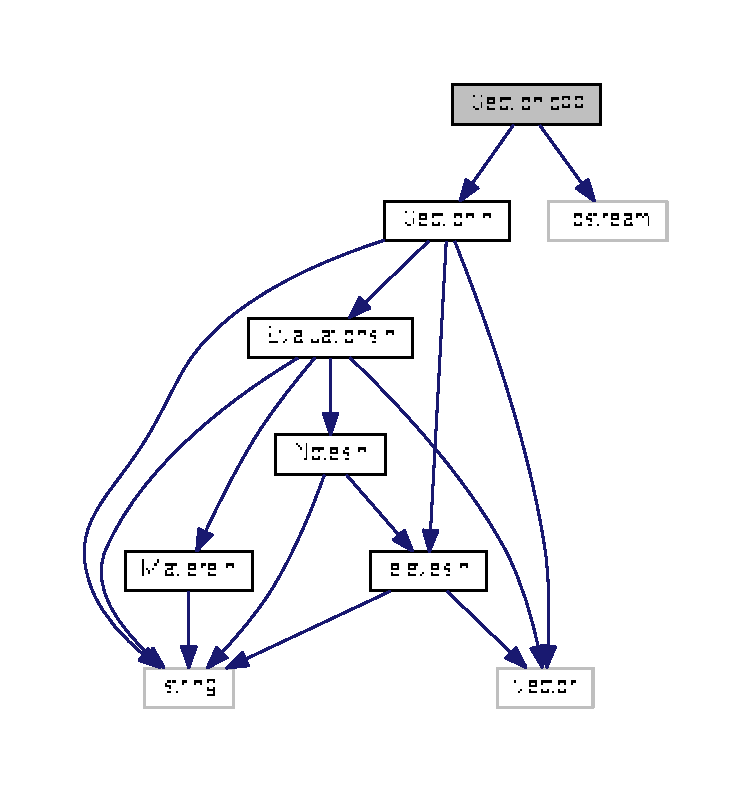
\includegraphics[width=350pt]{_section_8cpp__incl}
\end{center}
\end{figure}

\hypertarget{_section_8h}{\section{Section.\+h File Reference}
\label{_section_8h}\index{Section.\+h@{Section.\+h}}
}
{\ttfamily \#include $<$string$>$}\\*
{\ttfamily \#include $<$vector$>$}\\*
{\ttfamily \#include \char`\"{}eleves.\+h\char`\"{}}\\*
{\ttfamily \#include \char`\"{}Evaluations.\+h\char`\"{}}\\*
Include dependency graph for Section.\+h\+:\nopagebreak
\begin{figure}[H]
\begin{center}
\leavevmode
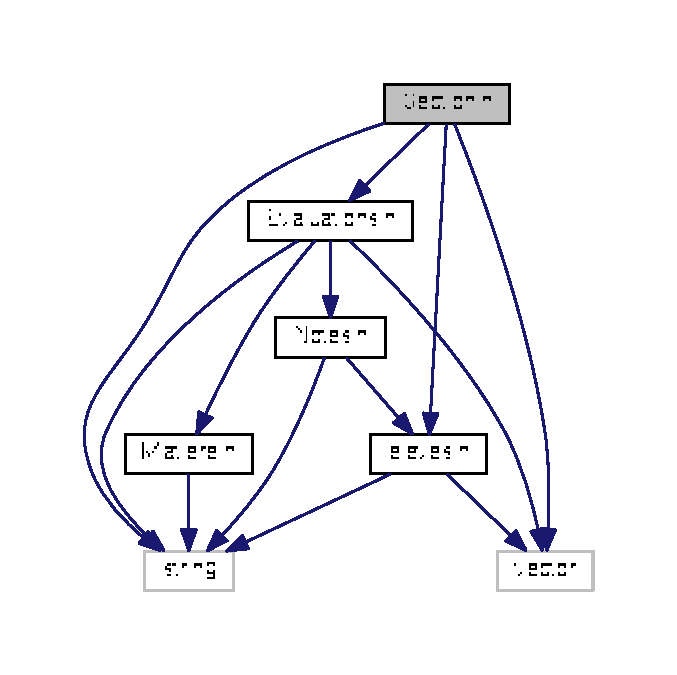
\includegraphics[width=325pt]{_section_8h__incl}
\end{center}
\end{figure}
This graph shows which files directly or indirectly include this file\+:\nopagebreak
\begin{figure}[H]
\begin{center}
\leavevmode
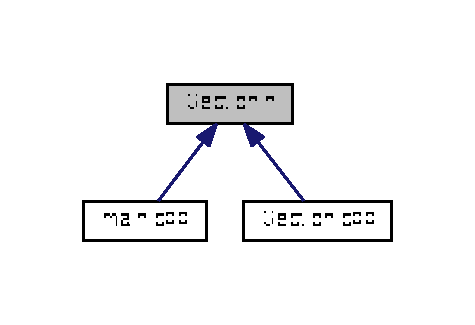
\includegraphics[width=228pt]{_section_8h__dep__incl}
\end{center}
\end{figure}
\subsection*{Classes}
\begin{DoxyCompactItemize}
\item 
class \hyperlink{class_section}{Section}
\end{DoxyCompactItemize}

%--- End generated contents ---

% Index
\newpage
\phantomsection
\addcontentsline{toc}{chapter}{Index}
\printindex

\end{document}
